% ===================================================================== CHƯƠNG 6
\chapter{Nguyên mẫu}\label{ch:nguyen-mau}

Chương này trả lời: nguyên mẫu làm được gì cho người dùng thật, chạy có ổn định không, cài đặt và tái lập có thuận tiện không, và còn những lỗi nào đã biết. Phần “làm được gì” được mô tả theo đúng trình tự công việc của một người soát xét.

\section{Phạm vi chức năng}

\begin{table}[htbp]
\centering
\caption{Phạm vi chức năng của nguyên mẫu (09–10/11/2026)}\label{tab:chuc-nang}
\bangchu
\rowcolors{2}{rowbg}{white}
\begin{tabularx}{\linewidth}{L{2.2cm}Y}
\hdr\thd{Trạng thái} & \thd{Chức năng}\\
Chạy được & Tải PDF, bản scan, văn bản và gán vai trò tài liệu; phân tích chạy nền có thanh tiến độ; trích tuyên bố, tìm bằng chứng, năm loại kết luận, chấm rủi ro, hàng đợi ưu tiên có lý do; xem trang gốc có tô sáng đoạn bằng chứng; thủ tục trên số liệu công bố (cộng lại bảng); ghi quyết định của người soát vào nhật ký chỉ ghi thêm, có lý do bắt buộc khi sửa kết luận; giấy làm việc tiếng Việt in được; xuất kết quả có cấu trúc, gói bằng chứng, bản kê tái lập và nhật ký; thư viện pháp lý; “Sửa báo cáo” gợi ý câu viết lại không thêm số, xuất DOCX có theo dõi thay đổi; trang hướng dẫn cho người mới\\
Sau cờ & Gói quy tắc tổ chức (có gói trình diễn của một ngân hàng giả lập); mô hình đọc cặp khó (đám mây hoặc GPU tại đơn vị); mô hình nhúng và xếp hạng lại\\
Chưa có & So sánh với kỳ trước và doanh nghiệp cùng ngành; phát hiện pháp lý tự động; dựng bảng PDF trong sản phẩm; đường đọc kép; xác thực người dùng nhiều cấp\\
\end{tabularx}
\end{table}

\section{Luồng làm việc của người soát xét}

Giao diện được tổ chức thành bốn bước, khớp với trình tự công việc thật.

\begin{enumerate}
\item \textbf{Tải tài liệu.} Người dùng tải báo cáo cần soát và tài liệu đối chiếu, chọn vai trò cho từng tài liệu, rồi bấm phân tích. Phân tích chạy nền, có thanh tiến độ theo bước, và nhãn “Ngoại tuyến – không gửi tài liệu ra ngoài” luôn hiện ở đầu trang.
\item \textbf{Soát theo hàng đợi.} Trang này trả lời câu hỏi “mở gì trước”. Đầu trang có bốn ô số: số mục nên soát trước, số mục đã chốt, số mục có đoạn mâu thuẫn, và độ phủ của bộ tài liệu. Danh sách chia bốn thẻ: cần soát, đã xem chưa chốt, đã chốt, ngoài hàng đợi. Mỗi mục ghi kết luận, tên tệp và số trang, kèm các nhãn ngắn giải thích vì sao mục được xếp lên: nhóm chỉ số, có số liệu không, thiếu mấy thuộc tính, có văn bản pháp lý liên quan không.
\item \textbf{Sửa báo cáo.} Câu tuyên bố được gạch dưới ngay trong văn bản. Người dùng chấp nhận, từ chối hoặc sửa từng gợi ý, rồi xuất DOCX có theo dõi thay đổi.
\item \textbf{Giấy làm việc.} Bản tổng hợp tiếng Việt in được, ghi phạm vi đã soát, phần cố ý chưa xét, các phép tính đã làm, quyết định của người soát và lý do.
\end{enumerate}

Trang chi tiết của một tuyên bố có các thẻ: thuộc tính, bằng chứng (kèm ảnh trang gốc có tô sáng), số liệu, pháp lý, rủi ro (phân rã chín thành phần) và xét duyệt. Ở thẻ xét duyệt, người soát chọn một trong các quyết định: xác nhận kết luận của máy, sửa kết luận, chưa kết luận được, hoặc yêu cầu thêm bằng chứng. Khi chọn “sửa kết luận”, giao diện bắt buộc chọn một trong bốn lý do (Bảng~\ref{tab:ly-do-sua}), và với lý do về quy tắc thì bắt buộc chỉ ra quy tắc. Ô ghi chú khuyến khích người soát viết lý do bằng lời, vì đó là phần người sau sẽ đọc lại.

\begin{figure}[htbp]
\centering
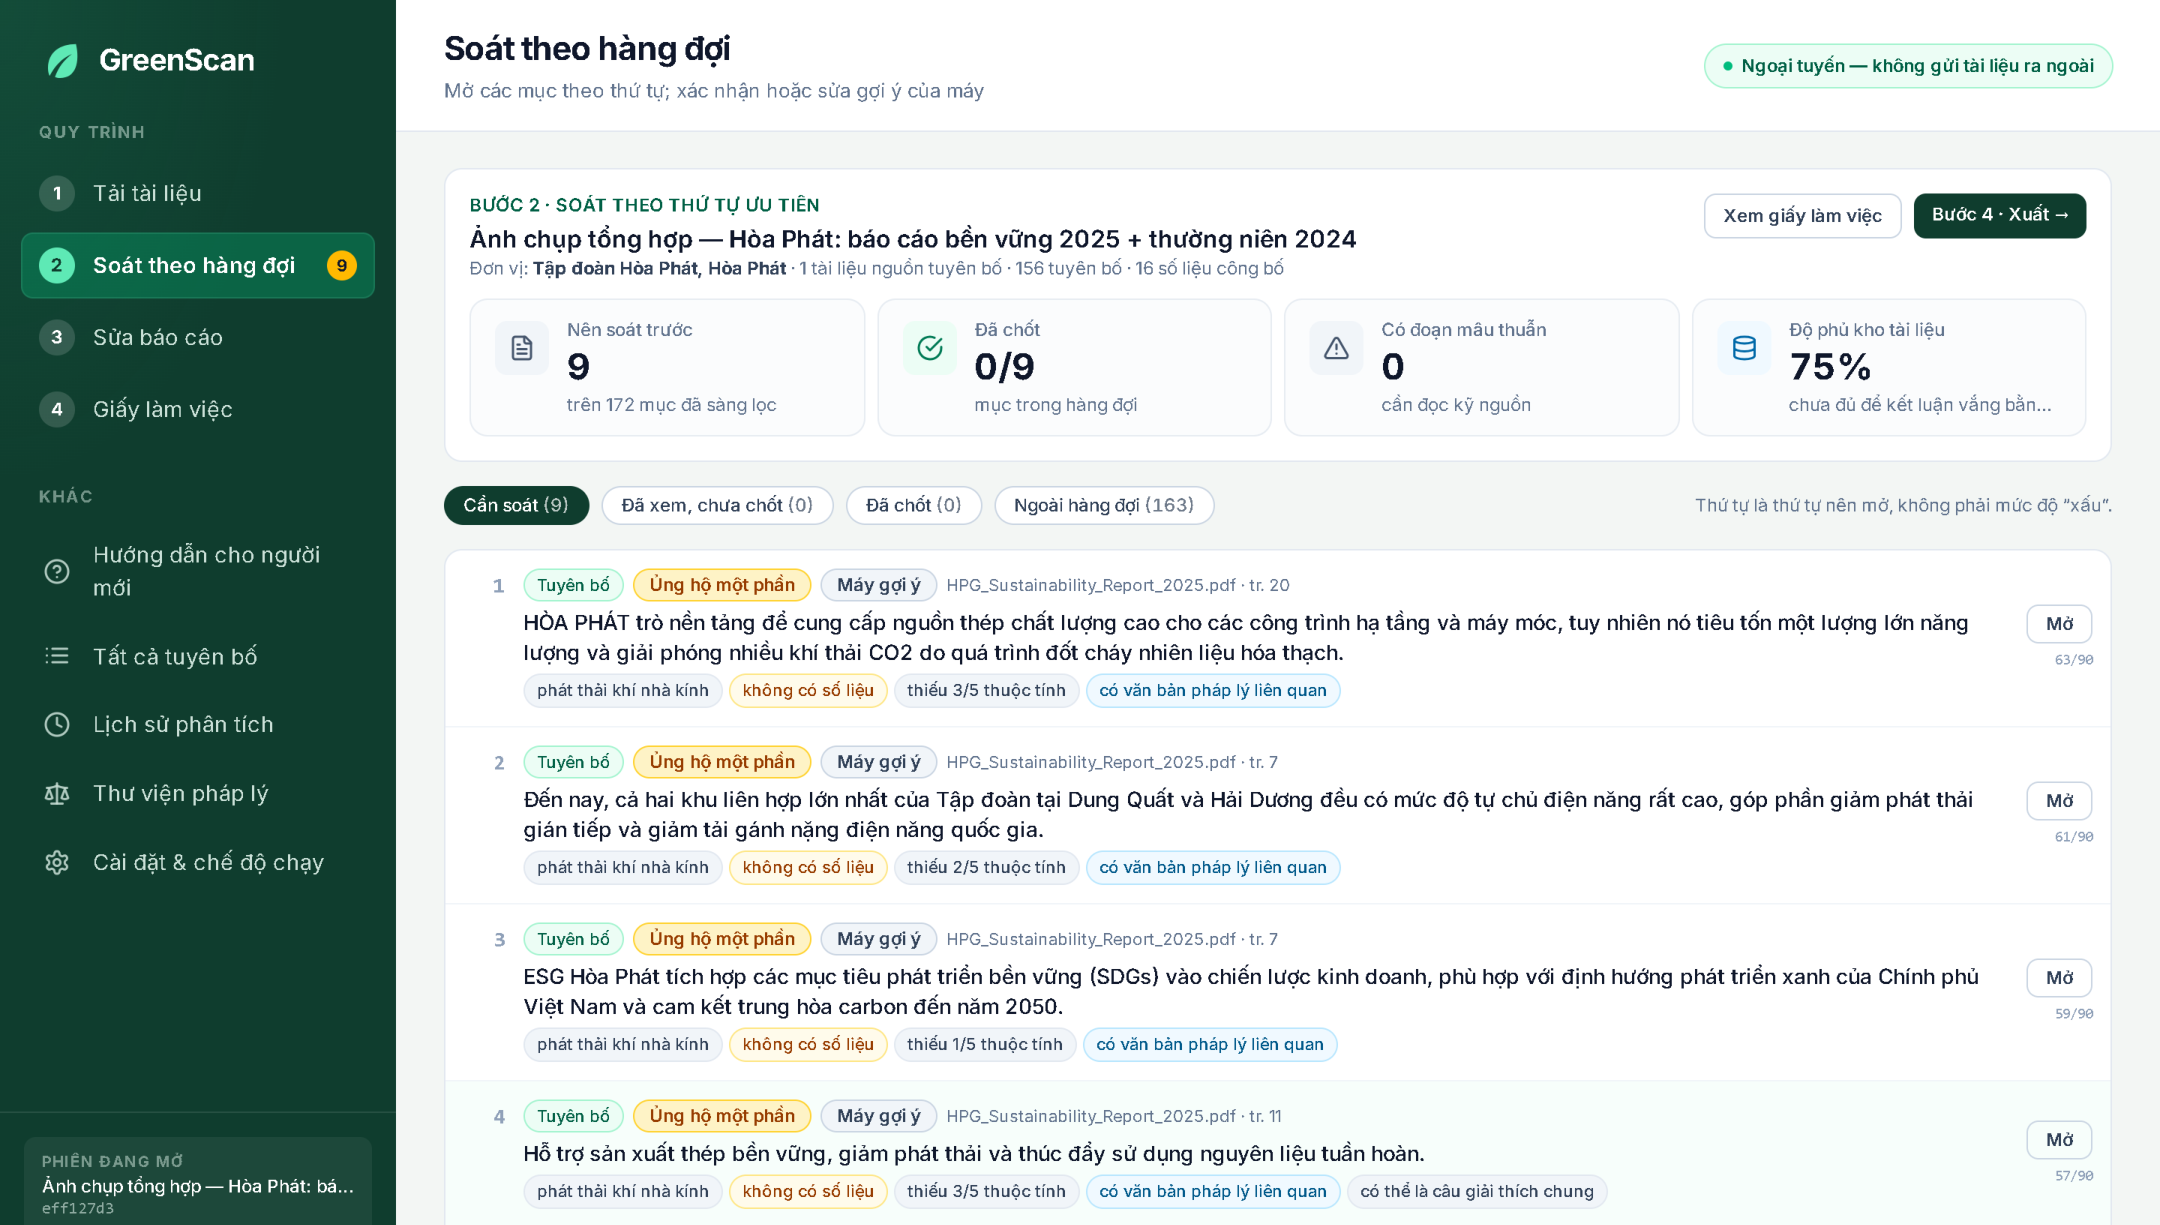
\includegraphics[width=\linewidth]{img/queue_top.png}
\caption[Trang “Soát theo hàng đợi” của phiên Hòa Phát]{Trang “Soát theo hàng đợi” của phiên Hòa Phát: 9 mục nên soát trước trên 172 mục đã sàng lọc, mỗi mục kèm lý do xếp hạng. Mục \#1 là một câu bị dính chữ khi đọc PDF, một lỗi đã biết được nêu ở mục~\ref{sec:loi-nguyen-mau}.}\label{fig:hang-doi}
\end{figure}

\subsection*{Kịch bản trình diễn}

Kịch bản trình diễn khoảng 3 phút, chạy trên phiên mẫu Hòa Phát cài sẵn để giám khảo không phải chờ:
\begin{enumerate}
\item mở phiên mẫu, hoặc tải hai tệp và chờ khoảng 2 phút;
\item vào bước “Soát theo hàng đợi”: 9/172 mục, đọc lý do xếp hạng;
\item mở mục \#2: xem năm thuộc tính, các đoạn bằng chứng và trang gốc có tô sáng;
\item xem thủ tục cộng lại bảng khí nhà kính trang 39;
\item ghi quyết định “yêu cầu thêm bằng chứng” kèm lý do;
\item mở giấy làm việc và in hoặc lưu PDF.
\end{enumerate}
Người xem quan sát được thứ tự mở, lý do xếp hạng, trang nguồn, phép tính, và cả phần mà lượt sàng lọc \emph{không} kiểm. Một video quay trực tiếp ứng dụng chạy ngoại tuyến (6 phút 31 giây) được chuẩn bị làm phương án dự phòng khi mạng hoặc máy chủ gặp sự cố.

\section{Ngôn ngữ giao diện và hướng dẫn người mới}

Người dùng mục tiêu là kiểm toán viên và chuyên viên tín dụng người Việt, nên giao diện chỉ dùng tiếng Việt. Nguyên tắc này được viết thành một chuẩn ngôn ngữ giao diện gồm năm nguyên tắc, bảng từ ngữ, tên năm loại kết luận và cách viết số, ngày. Mọi mã nội bộ đều có nhãn tiếng Việt. Chỉ giữ nguyên các ký hiệu chuẩn đã được công nhận rộng rãi như GRI hay tCO\textsubscript{2}e.

Chuẩn này được \emph{kiểm bằng máy}, không chỉ bằng mắt. Một công cụ quét chuỗi hiển thị, và một kiểm thử báo lỗi khi xuất hiện từ tiếng Anh hay mã mới. Các ngoại lệ đã duyệt (tên tệp, tên sản phẩm, dòng lệnh) được ghi vào một danh sách riêng.

Ở lần đăng nhập đầu, ứng dụng tự mở trang “Hướng dẫn cho người mới”. Trang này gồm bảy bước có thể đánh dấu, bảng năm loại kết luận, phần giải thích từ ngữ, và một mục riêng “GreenScan không làm gì”: không kết luận về doanh nghiệp, không kết luận vi phạm, không thay người soát.

\section{Hiệu năng và tài nguyên}

Trên laptop Intel i7-1355U, 16 GB RAM, không GPU, không khoá dịch vụ mô hình, bộ báo cáo Hòa Phát 264 trang được xử lý trong 107–154 giây qua các lần đo, RAM đỉnh 1,33 GB. Số này được đo bằng tiến trình con, lấy mẫu bộ nhớ mỗi 0,5 giây. Yêu cầu tối thiểu được khuyến nghị là 8 GB RAM. Trên máy chủ dùng chung, các lượt tải báo cáo mới được xếp hàng và chạy lần lượt.

\section{Kiểm thử và cổng hồi quy}

\begin{itemize}
\item \textbf{Bộ kiểm thử tự động}: 530 kiểm thử đạt, không có kiểm thử lỗi hay bị bỏ qua, khi chạy lại toàn bộ ngày 10/11/2026 (ngày 09/11 là 487; phần tăng thêm chủ yếu là kiểm thử cho việc ghi lý do khi sửa kết luận). Bộ này gồm kiểm thử đơn vị, đầu–cuối, 15 kiểm thử canh mười bất biến, 47 “bẫy kết luận” (mỗi lỗi từng gặp thành một bẫy), 17 ca theo danh mục kiểm tra của kiểm toán viên, kiểm thử luật an toàn của gói quy tắc, 6 kiểm thử chốt chặn mâu thuẫn, và kiểm thử ngôn ngữ giao diện.
\item \textbf{Cổng hồi quy cho mọi lần sửa đổi kết luận}: giữ nguyên 453/453 nhãn của GS-Bench v1.1 và 4/4 vụ có phán quyết; mọi kiểm thử bất biến phải đạt.
\item \textbf{Định nghĩa “xong”}: mỗi thay đổi phải trả lời bốn câu. Điều gì xảy ra khi thiếu bằng chứng? Điều gì xảy ra khi đầu vào không so được? Thay đổi có thể làm tăng kết luận “mâu thuẫn” sai không? Có quyết định nào bị chuyển từ luật sang mô hình không?
\end{itemize}

Số lượng kiểm thử không phải là bằng chứng về chất lượng phán đoán. Chất lượng được đo bằng các bộ đo ở Chương~\ref{ch:ket-qua}. Kiểm thử chứng minh một điều khác: các bảo đảm đã viết thành mã không bị phá khi mã thay đổi.

\section{Cài đặt, tái lập và đóng gói}

\begin{itemize}
\item \textbf{Cài trên Windows}: chỉ cần Python 3.11 và nhấp đúp tệp khởi động. Ứng dụng chạy giao diện và API trên cùng một cổng tại máy (127.0.0.1:8000). Trên Linux hoặc macOS có tệp khởi động tương ứng.
\item \textbf{Máy chủ}: có tệp Docker, chạy bằng người dùng không có quyền quản trị. Lớp mật khẩu cho bản chạy thử và trần dung lượng tệp tải lên đã có. Phiên mẫu Hòa Phát được tự cài khi khởi động, để giám khảo xem ngay. Việc dựng ảnh Docker \emph{chưa được thử lại} trong phiên làm việc ngày 09/11/2026.
\item \textbf{Tái lập}: mỗi lượt chạy ghi bản kê gồm mã băm tài liệu đầu vào, phiên bản cấu hình, phiên bản bộ quy tắc và lời nhắc. Cấu hình nằm trong tệp có số phiên bản. Chạy lại với cùng đầu vào cho cùng kết quả.
\item \textbf{Đóng gói nộp bài}: công cụ đóng gói quét khoá bí mật và tạo danh mục mã băm SHA-256 cho từng tệp. Công cụ này phải được chạy lại sau lần sửa mã cuối cùng.
\end{itemize}

\section{Lỗi đã biết của nguyên mẫu}\label{sec:loi-nguyen-mau}

Các lỗi dưới đây được phát hiện khi quay video trình diễn và chụp lại toàn bộ giao diện. Chúng được liệt kê để người dùng và giám khảo không phải tự phát hiện.

\begin{table}[htbp]
\centering
\caption{Lỗi đã biết của nguyên mẫu}\label{tab:loi-nguyen-mau}
\bangchu
\rowcolors{2}{rowbg}{white}
\begin{tabularx}{\linewidth}{L{4.2cm}YL{3.2cm}}
\hdr\thd{Lỗi} & \thd{Mô tả} & \thd{Ảnh hưởng}\\
Chữ dính khi đọc PDF & Mục \#1 của hàng đợi Hòa Phát: chữ “HÒA PHÁT” ở đầu trang bị ghép vào giữa câu mô tả lò cao & Một mục không phải tuyên bố đứng đầu hàng đợi\\
Số thuộc tính thiếu không thống nhất & Mục \#2: hàng đợi ghi thiếu 1/5, thẻ thuộc tính ghi 2/5, dòng tóm tắt ghi thiếu số liệu, kỳ và năm gốc & Người soát có thể bối rối\\
Tên kết luận không thống nhất & Hàng đợi ghi “ủng hộ một phần”, trang “Sửa báo cáo” ghi “khớp một phần” cho cùng kết luận & Gây hiểu nhầm nhẹ\\
Múi giờ & Lịch sử quyết định dùng giờ địa phương; nhật ký thay đổi và giấy làm việc dùng giờ UTC, không ghi chú & Khó đối chiếu thời điểm\\
Mã và cách viết số còn sót & Một số mã tiếng Anh còn hiện ở vài màn hình; số trong thủ tục cộng bảng viết theo kiểu Anh & Trái chuẩn ngôn ngữ giao diện\\
Bảng nhiều cột & Có thể đọc lẫn đơn vị hoặc dấu thập phân (ví dụ “7,085”) & Sai số liệu đọc ra\\
Màn hình hẹp & Trang “Sửa báo cáo” chưa co giãn ở bề ngang 390 px & Khó dùng trên điện thoại\\
Xác thực & Chưa có phân quyền nhiều cấp; bản chạy thử dùng một mật khẩu chung & Chưa đủ cho triển khai nhiều người dùng\\
\end{tabularx}
\end{table}

\FloatBarrier
\begin{hopy}{Tóm tắt chương}
\begin{itemize}
\item Nguyên mẫu là ứng dụng web chạy ngoại tuyến, đi theo bốn bước công việc của người soát: tải tài liệu, soát theo hàng đợi, sửa báo cáo, giấy làm việc.
\item Quyết định của người soát được ghi chỉ thêm; sửa kết luận thì phải chọn lý do, và lý do quyết định nhãn đi về mô hình hay về gói quy tắc.
\item 264 trang xử lý trong khoảng 2 phút trên laptop không GPU, RAM đỉnh 1,33 GB.
\item 530 kiểm thử đạt (10/11); cổng hồi quy giữ 453/453 nhãn ca dựng và 4/4 vụ có phán quyết. Giao diện chỉ tiếng Việt, được kiểm bằng máy.
\item Các lỗi đã biết (chữ dính, số thuộc tính không thống nhất, Docker chưa thử lại, chưa phân quyền) được nêu công khai.
\end{itemize}
\end{hopy}
